\documentclass[12pt]{article}

\usepackage{graphicx}
\usepackage{float}
\usepackage{amsmath}
\usepackage{amssymb}
\usepackage{graphicx}
\usepackage[utf8]{inputenc}
\usepackage[spanish]{babel}
\usepackage{geometry}
\geometry{left=2cm,right=2cm,top=2cm,bottom=2cm}
\usepackage{listings}
\lstset{basicstyle=\ttfamily,
  showstringspaces=false,
  commentstyle=\color{red},
  keywordstyle=\color{blue}
}


\title{%
  Scan Conversion\\
  \large Tarea 03 \\
    \Large Computación Gráfica\\
     \large UNAM 2022-2}
\author{Gibran Zazueta Cruz \\
\small 03/marzo/2022}
\date{}

\begin{document}
\maketitle

\section{Introducción}

Se programa el algoritmo de scan conversion para rellenar las caras de un cuboide.
El objeto y estructura de la escena es la misma que se utilizó para la tarea 2.


\subsection{Scan conversion}

\textit{Scan Conversion} es el proceso de convertir una figura geométrica o primitiva representada en el plano del dispositivo en un set de pixeles que describen su geometría. Esto incluye la representación de puntos, líneas, áres y figuras.
  
El nombre viene de que se 'escanea' la pantalla de arriba hacia abajo y de izquierda a derecha, para obtener la información de la primitiva.

\subsubsection{Rellenado de polígono
}

Para lograr rellenar un polígono primero se almacena la información de sus aristas en un \textit{Buffer}.


\begin{figure}[H]
\centering
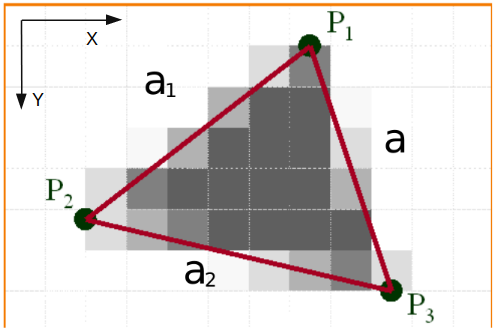
\includegraphics[scale=0.5]{images/scanfillED.png}
\caption{Algortimo rellenado de poligonos con Scan Conversion (imagen obtenida de \cite{fill})}
\end{figure}

Se siguen las aristas de la figura, una por una. Se calcula la pendiente de la recta y se va avanzando una unidad (de pixel) por \textit{y}, calculando el valor correspondiente para \textit{x}. Este proceso se debe realizar en orden, es decir, las aristas se siguen en orden horario o antihorario. 

Tomando como ejemplo la figura 2, un procesamiento antihorario sería: $a_{1} \rightarrow a_{2} \rightarrow a_{3}$.\\

La idea es dividir las aristas del polígono entre un 'lado izquierdo' y un 'lado derecho' que permita colorear los pixeles desde un borde hasta el otro, por cada coordenada $y$. 
Con un procesamiento de este tipo y para un polígono convexo el buffer almacenará 2 coordendas de $x$ por cada coordenada de $y$.\\

La manera en que se clasifican los bordes, entra parte derecha e izquierda, es tomando en cuenta el valor menor entre los dos vértices que forman la arista (por ejemplo $P_{1_{y}}$ y $P_{2_{y}}$ para la arista $a_{1}$).

Para un recorrido antihorario, mientras el valor del primer punto de la arista sea menor al del segundo se considera que esta pertenece al lado izquierdo. Cuando el valor del segundo punto de la arista sea menor al primero, la recta pertenece al lado derecho. 

La información de las coordendas $x$ (derecha e izquierda) correspondientes a cada coordenada $y$ se almacena en el buffer.\\

Una vez se tiene la información del buffer, se recorre la figura de arriba hacia abajo (tomando en cuenta el eje de coordenadas del dispostivo, esto corresponde a un incremento en  $y$), donde por cada valor de $y$ se colorean los pixeles desde la coordenada $x$ derecha hasta la $x$ izquierda.

Esta implementación´ está basada en la información presentada en \cite{bb}

\subsubsection{DDA}
Se utilizó el algortimo de Digital Differential analyzer para dibujar las lineas de las aristas del cubo. Este algoritmo necesita dos puntos (vértices) como entrada. Calcula los incrementos $\Delta X$, $\Delta Y$ . Finalmente su avanzan iterativamente las coordendas en incrementos $\Delta$, desde un punto inicial a un punto final, seleccionando en cada incremento el pixel a dibujar. 

\begin{figure}[H]
\centering
\includegraphics[scale=0.5]{images/DDA.png}
\caption{Algortimo DDA (imagen obtenida de \cite{dda})}
\end{figure}


  
\section{Estructura del código}

El programa tiene como base el código de la tarea 2.\\

En la clase CamProjection se programa el método de scan conversion para rellenar el poligono.

Después de proyectar y de pasar las coordenadas al plano del dispositivo, la función \textit{fillCubeFace()} recibe las coordenadas de cada una de las 6 caras del cubo (representadas por 4 vértices). Esta función llama a \textit{scanFillPoly()} que realiza el scan conversion, siguiendo cada una de las aristas y llenando el \textit{Buffer}, representado por un arreglo multidimensional.


Una vez completado el \textit{Buffer} se utiliza la información de este para ingresar los puntos a dibujar a la lista rasterPoints. Esta QList es la que finalmente se dibuja sobre el canvas.

El color de las caras se puede modificar en la clase renderWidow, can la variable pointPen. El color elegido es el blanco.

También en renderwindow se realizó una implementación de DDA en la función \textit{lineDDA()}

\section{Ejecutar el programa}
En la carpeta de build se puede ejecutar el programa con el archivo ScanConversion-Run. Desde la consola de comandos de linux:

\begin{lstlisting}[language=bash,title={bash}]
./ScanConversion-Run
\end{lstlisting}


En la carpeta principal está el código fuente. Para generar el ejecutable primero se genera el Makefile con

\begin{lstlisting}[language=bash,title={bash}]
 qmake ScanConversion.pro
\end{lstlisting}

Después se construye el proyecto con \textit{make}



\section{Instrucciones de uso}

\begin{figure}[H]
\centering
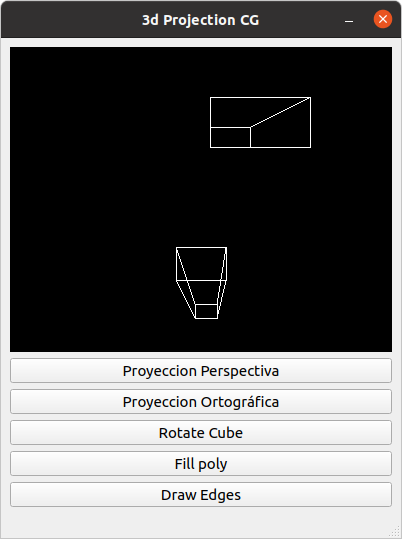
\includegraphics[scale=0.5]{images/gui.png}
\caption{Interfaz gráfica del programa}
\end{figure}

Se tienen los botones \textit{Fill poly} para rellenar las caras del cuboide y \textit{Draw edges} para dibujar sus aristas

El programa inicia sólo dibujando bordes. Al presionar \textit{Fill poly} se rellenarán las caras del polígono, al presionar una segunda vez se borrarán las caras. \textit{Draw Edges} funciona con un comportamiento similar


El boton \textit{Rotate cube} hace rotar el cubo sobre su eje x, de manera constante.
Los botones perspectiva y ortografica cambian a la proyeccion correspondiente.




\section{Programa en ejecución}

\begin{figure}[H]
\centering
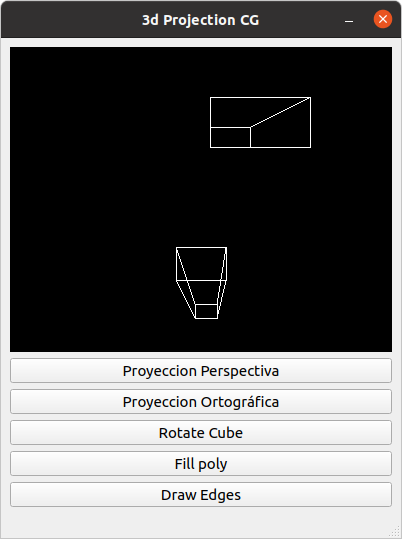
\includegraphics[scale=0.5]{images/gui.png}
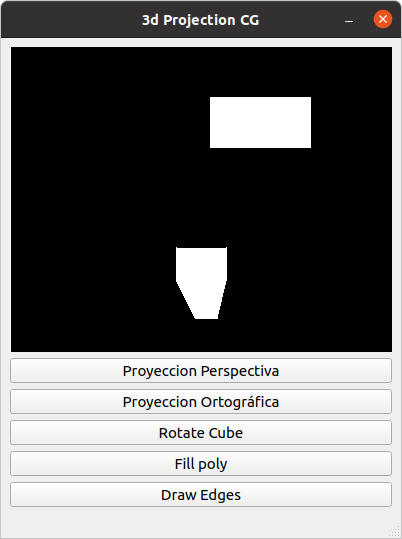
\includegraphics[scale=0.5]{images/ej2.png}
\caption{Cuboide con bordes y con rellenado. Proyectado en perspectiva}
\end{figure}

\begin{figure}[H]
\centering
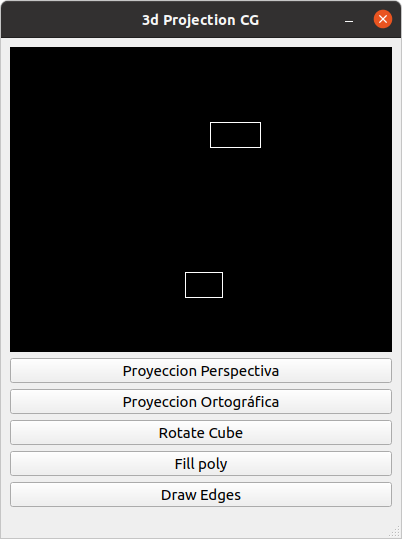
\includegraphics[scale=0.5]{images/ej1_ort.png}
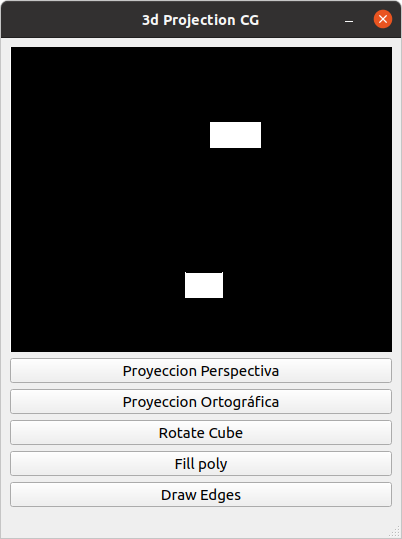
\includegraphics[scale=0.5]{images/ej2_ort.png}
\caption{Cuboide con bordes y con rellenado. Proyección Ortográfica}
\end{figure}


\begin{thebibliography}{99}


\bibitem{dda} Marchese. Image creation and Graphic primitives ($https://csis.pace.edu/~marchese/CG_Rev/L4/cg_l4.htm$)

\bibitem{fill} Funkhouser. 2D rendering Pipeline ($https://www.cs.princeton.edu/courses/$$\\$$archive/fall99/cs426/lectures/pipeline$)

\bibitem{bb} Upssala Universit. Introduction to polygons. ($http://www.it.uu.se/edu/course/homepage$\\$/grafik1/ht06/Lectures/L02/LinePolygon/x_polyd.htm$)

\end{thebibliography}


\end{document}